\documentclass[11pt,a4paper,titlepage]{article}

\usepackage[pdftex]{graphicx}
\usepackage{epstopdf}
\usepackage{subfigure}
\usepackage{amsmath,amsthm}
\usepackage{tikz}
\usetikzlibrary{babel}
\usetikzlibrary{shapes, arrows}
\textwidth= 15cm
\evensidemargin=0cm
\usepackage[english]{babel}
\usepackage[utf8]{inputenc}
\usepackage{textcomp}
\usepackage{amstext}
\usepackage{amsfonts}
\usepackage{amssymb}
\usepackage[hyperindex=true,breaklinks=true,colorlinks=true,linkcolor=blue]{hyperref}


\title{Brief course on the control of linear systems}
\author{Hector Garcia de Marina}

\tikzstyle{block} = [draw, rectangle, minimum width=6em]
\tikzstyle{sum} = [draw, fill=blue!20, circle, node distance=1cm]
\tikzstyle{input} = [coordinate]
\tikzstyle{output} = [coordinate]
\tikzstyle{pinstyle} = [pin edge={to-,thin,black}]

\newtheorem{definition}{Definition}
\newtheorem{theorem}{Theorem}
\newtheorem{algo}{Algorithm}
\newtheorem{remark}{Remark}


\begin{document}
\maketitle
\tableofcontents
\newpage
\section{State-space systems}
We will focus on systems that can be described by quantifiable characteristics or states, e.g., temperature, velocity or voltage. These states might change over time. One might interact with a system via a quantifiable input, and one might measure some information from the states of the system via a quantifiable output.

Let us define $x(t)\in\mathbb{R}^n$, $y(t)\in\mathbb{R}^m$ and $u(t)\in\mathbb{R}^k$ as the stacked (signal) vector of states, the output, and the input of a system $\Sigma$ respectively. In particular, we will describe them as continuous signals over time, e.g., $x(t) :[0,\infty) \to \mathbb{R}^n$. We can represent the system $\Sigma$ as a block with input/output ports and the states \emph{evolving inside} as it is shown in Figure \ref{fig: sigma}.

The system $\Sigma$ can be seen as a model that predicts the value of the states and the output over time given an input. This prediction incorporates the impact of the input (possibly zero) on the states and the output. We utilize differential equations as a tool to predict the evolution of the states of the system $\Sigma$ over time as follows
\begin{equation}
	\Sigma := \begin{cases}
		\dot x(t) =& f(x(t),u(t)) \\ y(t) =& g(x(t),u(t))
	\end{cases}, 
\label{eq: sigma}
\end{equation}
where $\dot x := \frac{\mathrm{d}}{\mathrm{dt}}(x(t))$ is the short notation for total derivative with respect to time, and $f: \mathbb{R}^n \times \mathbb{R}^k \to \mathbb{R}^n$ and $g: \mathbb{R}^n \times \mathbb{R}^k \to \mathbb{R}^m$ are arbitrary functions.



\begin{figure}[!h]
\centering
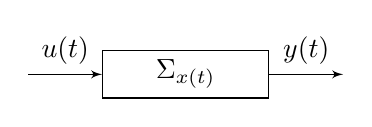
\begin{tikzpicture}[auto, node distance=2cm,>=latex']
	\node [input, name=input] {};
	\node [block, right of=input] (system) {$\Sigma_{x(t)}$};
	\node [output, right of=system] (output) {};
	\draw [draw,->] (input) -- node {$u(t)$} (system);
	\draw [->] (system) -- node [name=y] {$y(t)$}(output);
\end{tikzpicture}
	\caption{Input/output block diagram of system $\Sigma$.}
	\label{fig: sigma}
\end{figure}

\subsection{Example: Inverted pendulum}

We are going to find out the functions $f$ and $g$ for the inverted pendulum.

First, we derive the equations of motion of the mass in the inverted pendulum system in Figure \ref{fig: invpen} as a first step to figure out the system's functions $f$ and $g$. Consider that we can interact with the system with a torque $T$ applied on the base, the mass is under a friction force proportional to its speed, and we can only measure the angle $\theta$ from the system.

\begin{figure}[!h]
\centering
	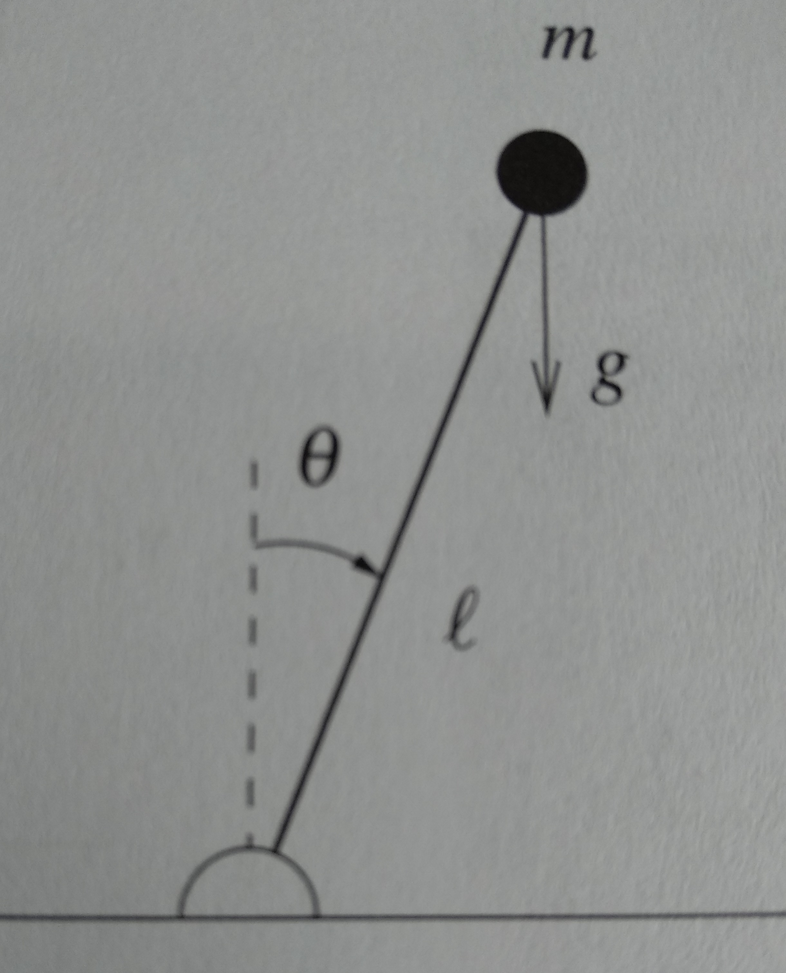
\includegraphics[scale=0.1]{./invpen.png}
	\caption{Inverted pendulum}
	\label{fig: invpen}
\end{figure}

We choose the angle $\theta$ with respect to the vertical to derive the dynamics of the inverted pendulum. Define $m, l, g,$ and $I\in\mathbb{R}$ as the mass, pendulum's lenght, gravity acceleration and inertia moment respectively. In particular, we have that $I = ml^2$, and we will exploit that $I \ddot\theta$ equals the sum of torques. We have to consider three torques; namely: 1. Torque $T$ applied by us; 2. Torque $-b\dot\theta$ applied by the friction; 3. Torque $mgl \sin\theta$ applied by the gravitational forces, i.e., $mg$ is the force on the mass, times $\sin\theta$ since the force only applies perpendicular to the bar, and times $l$ to compute the resultant torque. Therefore the dynamics of the inverted pendulum are given by
\begin{equation}
\ddot\theta = \frac{1}{ml^2}\left(mgl\sin{\theta}-b\dot\theta + T\right).
	\label{eq: dyn}
\end{equation}

It looks reasonable to choose $\theta$ as one of our states to construct $x(t)$. In fact, since we have derived a second-order system, we will need $\dot\theta$ as a second state since we have the differential equation for its time derivative $\ddot\theta$. Thus, let us define the state vector
\begin{equation}
x := \begin{bmatrix}\theta \\ \dot\theta \end{bmatrix},
\end{equation}
and since the torque $T$ is how we interact with the system, we choose the input $u(t) = T(t)$.

Now we are ready to construct the functions $f$ and $g$ in (\ref{eq: sigma}) for the inverted pendulum. In particular, we know that $f$ and $g$ only accepts as inputs/arguments the state space vector $x$ and the input $u$. On the left side of (\ref{eq: sigma}) we have the time derivative of $x(t)$, therefore
\begin{equation}
	\frac{\mathrm{d}}{\mathrm{dt}}\left(\begin{bmatrix}\theta \\ \dot\theta \end{bmatrix}\right) = f(x(t), u(t)) = \begin{bmatrix}f_1(x(t), u(t)) \\ f_2(x(t), u(t))\end{bmatrix}, \label{eq: fn}
\end{equation}
where $f_1(x) = \dot\theta$. Note that for the first row in (\ref{eq: fn}), on the left we have $\frac{\mathrm{d}}{\mathrm{dt}}\theta$, and on the right $f_1(x) = \dot\theta$ because $\dot\theta$ is actually a state, roughly speaking we can say that $\dot\theta(t) \in x(t)$. Unfortunately, we cannot say that $f_2(x) = \ddot\theta(t)$ because (roughly speaking) $\ddot\theta(t) \notin x(t)$. Nevertheless, we have that $f_2(x)$ is given by the differential equation (\ref{eq: dyn}). Then, let us write explicitly $f(x)$ as follows
\begin{equation}
	\frac{\mathrm{d}}{\mathrm{dt}}\left(\begin{bmatrix}\theta \\ \dot\theta \end{bmatrix}\right) =  f(x(t), u(t)) = \begin{bmatrix} \dot\theta \\ \frac{1}{ml^2}\left(mgl\sin{\theta}-b\dot\theta + T\right) \end{bmatrix}, \label{eq: f}
\end{equation}

The calculation of $g$ is more straightforward. We have established that we can only measure the angle, therefore $y(t) = \theta(t)$, i.e.,
\begin{equation}
g(x(t),u(t)) =  \theta(t).
	\label{eq: g}
\end{equation}

%A Python simulation of this dynamics can be found at \url{https://github.com/noether/aut_course}.

\section{Linearization of state-space systems}
Unfortunately, it is really (really) hard to calculate the analytic solution of $x(t)$ and $y(t)$ for a generic system $\Sigma$. Nevertheless, we will see that we can find the analytic solution for a state-space linear system.

The question, then, is whether we can relate a generic $\Sigma$ to a state-space linear system.

If $f(x,t)$ and $g(x,t)$ are real analytic around a specific point $(x^*,u^*)$, then, we can approximate them around $(x^*,u^*)$ by a Taylor series expansion. This approximation is what we call \emph{linearization} if we stop at order one in the Taylor series
\begin{align}
	\Sigma := \begin{cases}
	\dot x(t) =& f(x(t),u(t)) \\ y(t) =& g(x(t),u(t))
	\end{cases} \approx&
	\begin{cases}
	\delta \dot x(t) &= A(t)\delta x(t) + B(t)\delta u(t) \\
	\delta y(t) &= C(t)\delta x(t) + D(t)\delta u(t)
	\end{cases} \nonumber \\ \quad x(t) \approx& x^* + \delta x(t), \nonumber \\ u(t)\approx& u^* + \delta u(t), \nonumber \\
	y(t)\approx& y^* + \delta y(t), \quad y^*=g(x^*,u^*),\nonumber \\
\end{align}
where
\begin{align}
	A(t) &= \begin{bmatrix}
		\frac{\partial f_1}{\partial x_1} & \dots & \frac{\partial f_1}{\partial x_n} \\
		\vdots & \vdots & \vdots \\
		\frac{\partial f_n}{\partial x_1} & \dots & \frac{\partial f_n}{\partial x_n}
	\end{bmatrix}_{|_{x=x^*, u=u^*}} \nonumber \\
	B(t) &= \begin{bmatrix}
		\frac{\partial f_1}{\partial u_1} & \dots & \frac{\partial f_1}{\partial u_k} \\
		\vdots & \vdots & \vdots \\
		\frac{\partial f_k}{\partial u_1} & \dots & \frac{\partial f_k}{\partial u_k}
	\end{bmatrix}_{|_{x=x^*, u=u^*}} \nonumber \\
	C(t) &= \begin{bmatrix}
		\frac{\partial g_1}{\partial x_1} & \dots & \frac{\partial g_1}{\partial x_n} \\
		\vdots & \vdots & \vdots \\
		\frac{\partial g_m}{\partial x_1} & \dots & \frac{\partial g_m}{\partial x_n}
	\end{bmatrix}_{|_{x=x^*, u=u^*}} \nonumber \\
	D(t) &= \begin{bmatrix}
		\frac{\partial g_1}{\partial u_1} & \dots & \frac{\partial g_1}{\partial u_k} \\
		\vdots & \vdots & \vdots \\
		\frac{\partial g_m}{\partial u_1} & \dots & \frac{\partial g_m}{\partial u_k}
	\end{bmatrix}_{|_{x=x^*, u=u^*}} \nonumber
\end{align}
Roughly speaking, we calculate the sensitivity (up to first order) of $f$ and $g$ when we make a small variation on $x$ and $u$ around $(x^*,u^*)$. How close $(x,u)$ must be to $(x^*,u^*)$ depends on the particular system $\Sigma$. Later in Section \ref{sec: sta}, we will provide bounds for $\delta x$ and $\delta u$ such that we can apply with guarantees our control algorithms.

\subsection{Example: Inverted pendulum}
We will see that, with the linearization, we can design controllers $u(t)$, i.e., a signal that our torque $T$ must follow, to drive the state of the pendulum where we wish. Let us define this point of interest as $x^* = \begin{bmatrix}\theta^* \\ 0\end{bmatrix}$, i.e., a fixed angle with (obviously) zero velocity. Indeed, this is an equilibrium point for the angle $\theta$. In order to have an equilibrium, we need to find an input $u(t)$ in (\ref{eq: f}) such that $\frac{\mathrm{d}}{\mathrm{dt}}\left(\begin{bmatrix}\theta \\ \dot\theta \end{bmatrix}\right) = \begin{bmatrix}0 \\ 0 \end{bmatrix}$. A quick inspection to the dynamics (\ref{eq: dyn}) we have that
\begin{equation}
	u^* = T^* = -\frac{g}{l}\sin\theta^*,
\end{equation}
for example, for the vertical position of the pendulum corresponding to $\theta^* = 0$, we have that $T^*=0$, i.e., $x^* = \begin{bmatrix}0\\0\end{bmatrix}$ and $u^* = 0$.

The calculation of the matrices $A,B,C,$ and $D$ are the corresponding Jacobians for $(\ref{eq: f})$ and $(\ref{eq: g})$, i.e.,

\begin{align}
\frac{\partial f_1}{\partial x_1} &= 0 \nonumber \\
\frac{\partial f_1}{\partial x_2} &= 1 \nonumber \\
\frac{\partial f_2}{\partial x_1} &= \frac{g}{l}\cos\theta \nonumber \\
\frac{\partial f_2}{\partial x_2} &= -\frac{b}{ml^2} \nonumber \\
\frac{\partial f_1}{\partial u_1} &= 0 \nonumber \\
\frac{\partial f_2}{\partial u_1} &= 1 \nonumber \\
\frac{\partial g_1}{\partial x_1} &= 1 \nonumber \\
\frac{\partial g_1}{\partial x_2} &= 0 \nonumber \\
\frac{\partial g_1}{\partial u_1} &= 0, \nonumber
\end{align}
therefore we can arrive at
\begin{align}
	\frac{\mathrm{d}}{\mathrm{dt}}\left(\begin{bmatrix}\delta\theta \\ \dot\delta\theta \end{bmatrix}\right) &= \begin{bmatrix}0 & 1 \\ \frac{g}{l}\cos\theta & -\frac{b}{ml^2} \end{bmatrix}_{|_{\theta=\theta^*}} \begin{bmatrix}\delta\theta \\ \dot\delta\theta \end{bmatrix} + \begin{bmatrix}0 \\ 1 \end{bmatrix} \delta T \nonumber \\
		\delta y &= \begin{bmatrix}1 & 0\end{bmatrix}\begin{bmatrix}\delta\theta \\ \dot\delta\theta \end{bmatrix} + 0 \, \delta T,
\end{align}
to model the dynamics of $x(t)$ and the output $y(t)$ around the points $x^*$ and $u^*$.

\section{Solution to Linear State-Space systems}
We call linear state-space system to the following particular linear system
\begin{equation}
	\Sigma_{\text{linear}} := \begin{cases}
	\dot x(t) &= A(t)x(t) + B(t)u(t) \\
	 y(t) &= C(t)x(t) + D(t)u(t)
	\end{cases},
\label{eq: sigmalin}
\end{equation}
where $A(t)\in\mathbb{R}^{n\times n},B(t)\in\mathbb{R}^{n\times k},C(t)\in\mathbb{R}^{n\times m}$ and $D(t)\in\mathbb{R}^{k\times m}$ are possibly time-varying matrices.

The solution to an \emph{ordinary differential equation} (ODE) is given by the addition of two terms: the solution to the homogeneous part, and a particular solution to the non-homogeneous.

\begin{equation}
	\dot x(t) = \underbrace{A(t)x(t)}_{\text{homogeneous}} + \underbrace{B(t)u(t)}_{\text{non-homogeneous}}
	\label{eq: xdyn}
\end{equation}

\begin{theorem}{Peano-Barker series:}
The unique solution to the homogeneous $\dot x = Ax$ is given by
	\begin{equation}
		x(t) = \Phi(t,t_0)x(t_0), \quad x(t_0)\in\mathbb{R}^n, t\geq 0,
	\end{equation}
where
	\begin{align}
		\Phi(t,t_0) := I + \int_{t_0}^t A(s_1)ds_1 + \int_{t_0}^t A(s_1) \int_{t_0}^{s_1} A(s_2)ds_2ds_1 \nonumber \\ + \int_{t_0}^t A(s_1) \int_{t_0}^{s_1} A(s_2)\int_{t_0}^{s_2} A(s_3) ds_3ds_2ds_1 + \dots . \label{eq: ser}
	\end{align}
\end{theorem}
Sketch of the proof:
First, we note that
\begin{equation}
	\frac{\mathrm{d}}{\mathrm{dt}} \int_a^t f(t,s)ds = f(t,t) + \int_a^t \frac{\partial f(t,s)}{\partial t}ds.
\end{equation}

Then, we calculate the following time derivative
	\begin{align}
		\frac{\mathrm{d}}{\mathrm{dt}}\Phi(t,t_0) &= A(t) + A(t)\int_{t_0}^{t}A(s_2)ds_2 \nonumber \\ &+ A(t)\int_{t_0}^t A(s_2) \int_{t_0}^{s_2} A(s_3)ds_3ds_2 + \dots \nonumber \\
		&= A(t) \Phi(t,t_0).
	\end{align}
We claim that the solution to the homogeneous part of (\ref{eq: xdyn}) is $x(t) = \Phi(t,t_0)x_0$ ($x_0$ is the short notation for $x(t_0)$), whose time derivative is given by
\begin{align}
	\frac{\mathrm{d}}{\mathrm{dt}} x(t) &= \frac{\mathrm{d}}{\mathrm{dt}}\left(\Phi(t,t_0)x_0\right) \nonumber \\
	&= A(t) \Phi(t,t_0) x_0 \nonumber \\
	&= A(t)x(t),
\end{align}
which is proving the identity $\dot x = A(t)x(t)$ given that $x(t) = \Phi(t,t_0)x_0$. In order to make this proof complete, we would need to prove that the series (\ref{eq: ser}) converges for $t\geq t_0$. That material should be covered in a standard course on differential equations.

The matrix $\Phi(t,t_0)$ is called the \textbf{\emph{state transition matrix}}. Given an initial condition $x_0$, we can predict $x(t)$ in (\ref{eq: xdyn}) given that we do not interact with the system, i.e., $u(t) = 0, t\geq t_0$.

\subsection{Solution to the homogenous + nonhomogenous}
The unique solution to (\ref{eq: sigmalin}) applying the \emph{variation of constants} method is given by:
\begin{align}
	x(t) &= \Phi(t,t_0)x_0 + \int_{t_0}^t \Phi(t,\tau)B(\tau)u(\tau)d\tau \label{eq: solx} \\
	y(t) &= C(t)\Phi(t,t_0)x_0 + \int_{t_0}^t C(t)\Phi(t,\tau)B(\tau)u(\tau)d\tau + D(t)u(t). \label{eq: soly}
\end{align}

\subsection{Solution to Linear Time Invariant Systems}

The matrix $\Phi(t,t_0)$ can be calculated analytically when $A$ is a matrix with constant coefficients. If $A$ is constant, we can take it out from the integrals in (\ref{eq: ser})
\begin{align}
	\Phi(t,t_0) := I + A \int_{t_0}^t ds_1 + A^2 \int_{t_0}^t \int_{t_0}^{s_1} ds_2ds_1 \nonumber \\ + A^3 \int_{t_0}^t \int_{t_0}^{s_1} \int_{t_0}^{s_2} ds_3ds_2ds_1 + \dots \label{eq: phi},
\end{align}
and noting that the following integrals can be easily solved
\begin{align}
	\int_{t_0}^t ds_1 &= (t-t_0) \nonumber \\
	\int_{t_0}^t\int_{t_0}^{s_1} ds_2ds_1 &= \frac{(t-t_0)^2}{2} \nonumber \\
	\vdots \nonumber \\
	\int_{t_0}^t\int_{t_0}^{s_1} \cdots \int_{t_0}^{s_{k-2}}\int_{t_0}^{s_{k-1}}ds_k ds_{k-1} \cdots ds_2ds_1 &= \frac{(t-t_0)^k}{k!}, \nonumber
\end{align}
then we have that (\ref{eq: phi}) can be calculated by
\begin{equation}
	\Phi(t,t_0) = \sum_{k=0}^{\infty} \frac{(t-t_0)^k}{k!}A^k,
\end{equation}
which resembles to the power series of the scalar exponential function, i.e., $e^x := \sum_{k=0}^{\infty}\frac{1}{k!}x^k = 1 + x + \frac{x^2}{2} + \frac{x^3}{3!} + \dots $. In fact, the definition of the \emph{exponential of a matrix} is
\begin{equation}
	exp(A) = I + A + \frac{1}{2} A^2 + \frac{1}{3!} A^3 + \dots
\end{equation}

Let us set $t_0 = 0$ for the sake of convenience, then
\begin{align}
	\Phi(t,0) &= I + tA + \frac{t^2}{2} A^2 + \frac{t^3}{3!} A^3 + \dots \nonumber \\
	&= exp(At),
\end{align}
therefore the solution to the homogeneous (\ref{eq: xdyn}) with $A$ constant and setting $t_0 = 0$ is
\begin{equation}
	x(t) = exp(At)x_0,\quad t\geq 0.
	\label{eq: xexp}
\end{equation}

To continue further, we need the following result from Linear Algebra.
\begin{theorem}
\textbf{Jordan Form}. For every square matrix $A\in\mathbb{C}^{n \times n}$, there exists a non-singular change of basis matrix $P\in\mathbb{C}^{n \times n}$ that transforms $A$ into
\begin{equation}
	J = PAP^{-1} = \begin{bmatrix}
		J_1 & 0 & 0 & \dots & 0 \\
		0 & J_2 & 0 & \dots & 0 \\
		0 & 0 & J_3 & \dots & 0 \\
		\vdots & \vdots & \vdots & \cdots & \vdots \\
		0 & 0 & 0 & \cdots & J_l
	\end{bmatrix},
\end{equation}
where each $J_i$ is a Jordan block of the form
	\begin{equation}
	J_i = \begin{bmatrix}
\lambda_i & 1 & 0 & \dots & 0 \\
		0 & \lambda_i & 1 & \dots & 0 \\
		0 & 0 & \lambda_i & \dots & 0 \\
		\vdots & \vdots & \vdots & \cdots & \vdots \\
		0 & 0 & 0 & \cdots & \lambda_i
	\end{bmatrix}_{n_i\times n_i},
	\end{equation}
	where each $\lambda_i$ is an eigenvalue of $A$, and the number $l$ of Jordan blocks is equal to the total number of independent eigenvectors of $A$. The matrix $J$ is unique up to a reordering of the Jordan blocks and is called the \textbf{Jordan normal form} of $A$.
\end{theorem}

Note that $A = P^{-1}JP$ as well, and we leave as an exercise to prove that
\begin{equation}
	A^k = P^{-1} J^k P,
\end{equation}
so we can calculate
\begin{align}
	exp(At) &= P^{-1}\left(\sum_{k=0}^\infty \frac{t^k}{k!} \begin{bmatrix}J_1^k & 0 & \cdots & 0 \\ 0 & J_2^k & \cdots & 0 \\ \vdots & \vdots & \cdots & \vdots \\ 0 & 0 & \cdots & J_l^k \end{bmatrix} \right) P \nonumber \\
		&= P^{-1} \begin{bmatrix}exp(J_1t) & 0 & \cdots & 0 \\ 0 & exp(J_2t) & \cdots & 0 \\ \vdots & \vdots & \cdots & \vdots \\ 0 & 0 & \cdots & exp(J_lt) \end{bmatrix} P.
\end{align}

Therefore if $J$ is just a diagonal matrix with the eigenvalues of $A$, i.e., $J_l = \lambda_l \in \mathbb{C}$, then $exp(J_lt) = e^{\lambda_lt} \in\mathbb{C}$ is a trivial calculation.

In general, we have that
\begin{equation}
	exp(J_it) = e^{\lambda_i t}
	\begin{bmatrix}1 & t & \frac{t^2}{2!} & \frac{t^3}{3!} & \cdots & \frac{t^{n_i-1}}{(n_i-1)!} \\
		0 & 1 & t & \frac{t^2}{2!} & \cdots & \frac{t^{n_i-2}}{(n_i-2)!} \\
		0 & 0 & 1 & t & \cdots & \frac{t^{n_i-3}}{(n_i-3)!} \\
	\vdots & \vdots & \vdots & \ddots & \ddots & \vdots \\
	0 & 0 & 0 & 0 & \ddots & t \\
	0 & 0 & 0 & 0 & \cdots & 1
\end{bmatrix},
\end{equation}
where $n_i$ is the size of the corresponding Jordan block.

\subsubsection{Connection between the eigenvalues of $A$ and the $exp(At)$}
Now, let us check the consequences and connections between the eigenvalues of $A$ and the $exp(At)$:
\begin{enumerate}
	\item When all the eigenvalues of $A$ have strictly negative real parts, then all the $exp(J_it) \to 0$ as $t\to\infty$. Thus, $exp(At)\to 0 $ as $t\to\infty$.
	\item When all the eigenvalues of $A$ have negative or zero real parts and all the Jordan blocks corresponding to eigenvalues with zero real parts are $1\times 1$, then all the $exp(J_it)$ remain bounded as $t\to\infty$. Thus, $exp(At)\to 0 $ remains bounded as $t\to\infty$.
	\item When at least one eigenvalue of $A$ has a positive real part or a zero real part with the corresponding Jordan block bigger than $1\times 1$, then $exp(At)$ is unbounded as $t\to\infty$.
\end{enumerate}

\section{(Internal or Lyapunov) Stability}
\label{sec: sta}

We say that the linear system (\ref{eq: sigmalin}) \emph{in the sense of Lyapunov}
\begin{enumerate}
	\item is \emph{(marginally) stable} if for every initial condition $x_0$, then $x(t) = \Phi(t,t_0) x_0$ is uniformily bounded for all $t>t_0$.
	\item is \emph{asymptotically stable} if, in addition, $x(t) \to 0$ as $t\to\infty$.
	\item is \emph{exponentially stable} if, in addition, $||x(t)|| \leq c e^{\lambda(t-t_0)}||x(t_0)||$ for some constants $c,\lambda > 0$.
	\item is \emph{unstable} if it is not marginally stable.
\end{enumerate}

%In control, it is very common to focus on \emph{error signals}, e.g., $e(t) := x(t) - x^*(t)$, where $x^*(t)$ is a trajectory goal. Note that if $x^*$ is constant, then $\dot e(t) = \dot x(t)$, and this is why we focus on having $x(t) \to 0$ as $t\to\infty$ in the above definitions for (\ref{eq: sigmalin}).

Let us now check the particular case when $A$ is constant, i.e., $\Phi(t,t_0) = e^{A(t-t_0)}$. Then, we can stablish a clear relation between the eigenvalues of $A$ and the stability definitions in the sense of Lyapunov by inspecting the solution to $\dot x(t) = Ax(t)$ given by
\begin{equation}
	x(t) = \sum_{l=1}^n f_le^{\lambda_l t},
\label{eq: solptcom}
\end{equation}
where $\lambda_l$ are the eigenvalues of $A$, $f_l(t,c_l,\dots,c_n,w_l,\dots,w_n)$ are different functions corresponding to linear combinations like $c_lw_l + c_{l+1}(w_{l+1}+w_lt)+\dots$ depending on the (possibly generalized) eigenvectors $w_l$ associated to $\lambda_t$, and $c_l$ are constants determined by the initial condition $x(0)$. Note that for single eigenvalues we have that $f_l = w_l$.

The system $\dot x(t) = Ax(t)$
\begin{enumerate}
	\item is marginally stable if and only if all the eigenvalues of $A$ have negative real part or zero real parts (with all the Jordan blocks being $1\times 1$).
	\item is asymptotically (and equivalently exponentially) stable if and only if all the eigenvalues of $A$ have strictly negative real parts.
	\item is unstable if and only if at least one eigenvalues of $A$ has a positive real part or zero real part (with the corresponding Jordan block being larger than $1\times 1$).
\end{enumerate}

Checking the solution(s) to a linear system (\ref{eq: solx})-(\ref{eq: soly}) we can say that if $A$ is constant and $\dot x = Ax$ is asymptotically stable, then $x(t) \to \int_{t_0}^t e^{A(t-\tau)}B(\tau)u(\tau)d\tau$ as $t\to\infty$. 

\subsection{Stability of locally linearized systems}
The following equation is also equivalent to have asymptotic (exponential) stability for $\dot x(t) = Ax(t)$. There exists a unique solution $P$ for the following \emph{Lyapunov equation}
\begin{equation}
A^TP + PA = -Q, \quad \forall Q \succ 0.
	\label{eq: lya}
\end{equation}
You can prove (\ref{eq: lya}) by considering
\begin{equation}
	P:= \int_0^\infty e^{A^Tt}Qe^{At}dt.
	\label{eq: P}
\end{equation}
Hint: First, substitute $P$ in (\ref{eq: lya}), and then check the calculation $\frac{\mathrm{d}}{\mathrm{dt}}\left(e^{A^Tt}Qe^{At}\right)$. Since $P$ is unique, then $P$ must be positive definite according to its definition (\ref{eq: P}).

Let us consider an autonomous continuous-time nonlinear system
\begin{equation}
	\dot x(t) = f(x(t)), \quad x\in\mathbb{R}^n,
	\label{eq: non}
\end{equation}
with an equilibrium point $x^*\in\mathbb{R}^n$, i.e., $f(x^*) = 0$. The dynamics of $x(t)$ around $x^*$ can be approximated by considering $x(t) = x^* + \delta x(t)$ where
\begin{equation}
	\dot{\delta x(t)} = A\,\delta x(t), \quad A:=\frac{\partial f(x)}{\partial x}.
	\label{eq: delta}
\end{equation}

What is this approximation good for?

\begin{theorem}
	\label{thm: tayl}
	Assume that $f(x)$ is twice differentiable. If (\ref{eq: delta}) is exponentially stable, then there exists a neighborhood $\mathcal{B}$ around $x^*$ and constants $c, \lambda > 0$ such that for every solution $x(t)$ to the nonlinear system (\ref{eq: non}) that starts at $x(t_0)\in\mathcal{B}$, we have
	\begin{equation}
	||x(t) - x^*|| \leq ce^{\lambda(t-t_0)} ||x(t_0) - x^*||, \quad \forall t\geq t_0.
	\end{equation}
\end{theorem}

\subsubsection{How big is $\mathcal{B}$? Can we estimate it? Sketch of the proof of Theorem \ref{thm: tayl}}

Since $f$ is twice differentiable, from its Taylor's series we have that
\begin{equation}
	r(x) := f(x) - (f(x^*) + A(x - x^*)) = f(x) - A\,\delta x = O(||\delta x||^2),
\end{equation}
which means that there exist a constant $c$ and a ball $\bar B$ around $x^*$ such that
\begin{equation}
	||r(x)|| \leq c||\delta x||^2, \quad x\in\bar B.
\end{equation}
If the linearized system is exponentially stable, we have that
\begin{equation}
A^TP + PA = -I.
\end{equation}
Now consider the following scalar signal
\begin{equation}
	v(t) := (\delta x)^T P \delta x, \quad \forall t\geq 0.
\end{equation}
Noting that $\delta x(t) = x(t) - x^*$, then $\dot{\delta x(t)} = \dot x(t) = f(t)$. Therefore, the time derivative of $v(t)$ satisfies
\begin{align}
	\dot v &= f(x)^T P \delta x + (\delta x)^T P f(x) \nonumber \\
	&= (A\delta x + r(x))^T P \delta x + (\delta x)^T P (A\delta x + r(x)) \nonumber \\
	&= (\delta x)^T(A^T P + PA)\delta x + 2(\delta x)^T P r(x) \nonumber \\
	&= -||\delta x||^2 + 2(\delta x)^T P r(x) \nonumber \\
	&\leq -||\delta x||^2 + 2 ||P||\, ||\delta x|| \, ||r(x)||.
\end{align}

We have that $v(t)$ is positive excepting when $\delta x = 0$. If we can guarantee that $\dot v(t) < 0$ and $\dot v(t) = 0$ only when $\delta x = 0$, then $v(t) \to 0$ as $t\to\infty$, which means that $\delta x(t) \to 0$ as $t\to\infty$.

Now, if $x\in\mathcal{\bar B}$, then
\begin{equation}
	\dot v \leq -\Big(1 - 2c\,||P||\,||\delta x||\Big)||\delta x||^2,
\end{equation}
Thus, if the deviation $\delta x$ is small enough, i.e.,
\begin{equation}
||\delta x|| < \frac{1}{2c||P||},
\end{equation}
then $\dot v(t) < 0$ if $\delta x(0) \neq 0$ and $\delta x(0) < \frac{1}{2c||P||}$.

We can conclude that an estimation of $\mathcal B$ is
\begin{equation}
	\mathcal{B} := \{ \delta x : ||\delta x|| < \frac{1}{2c||P||} \}.
	\label{eq: Bregion}
\end{equation}

\section{Controllability}
\subsection{Reachable and Controllable subspaces}
We recall that when we apply an input $u(\cdot)$ to (\ref{eq: sigmalin}), we transfer the system from a state $x(t_0):=x_0$ to a state $x(t_1):=x_1$, and it is calculated from (\ref{eq: solx}) as follows
\begin{equation}
	x_1 = \Phi(t_1,t_0)x_0 + \int_{t_0}^{t_1} \Phi(t_1,\tau)B(\tau)u(\tau)d\tau,
\end{equation}
where $\Phi(\cdot)$ is the system's state transition matrix.

Questions: 
\begin{enumerate}
	\item Which states can I reach from $x_0$?
	\item Is there always an input $u(\cdot)$ that transfers the system from an arbirtrary state $x_0$ to another arbitrary state $x_1$?
\end{enumerate}

These two questions lead to the definition of the reachable and controllable subspaces.

\begin{definition}[Reachable subspace]
	Given two times $t_1>t_0\geq 0$, the reachable or controllable-from-the-origin on $[t_0,t_1]$ subspace $\mathcal{R}[t_0,t_1]$ consists of all the states $x_1$ for wichi there exists an input $u:[t_0,t_1]\to \mathbb{R}^k$ that transfers the state from $x_0 = 0$ to $x_1 \in\mathbb{R}^n$; i.e.,
	\begin{equation}
		\mathcal{R}[t_0,t_1] := \Big\{x_1\in\mathbb{R}^n : \exists u(\cdot),\, x_1 = \int_{t_0}^{t_1} \Phi(t_1,\tau)B(\tau)u(\tau)d\tau \Big\}. \label{eq: rs}
	\end{equation}
\end{definition}

\begin{definition}[Controllable subspace]
	Given two times $t_1>t_0\geq 0$, the controllable or controllable-to-the-origin on $[t_0,t_1]$ subspace $\mathcal{C}[t_0,t_1]$ consists of all the states $x_1$ for wichi there exists an input $u:[t_0,t_1]\to \mathbb{R}^k$ that transfers the state from $x_0\in\mathbb{R}^n$ to $x_1 = 0$; i.e.,
	\begin{equation}
		\mathcal{C}[t_0,t_1] := \Big\{x_0\in\mathbb{R}^n : \exists u(\cdot),\, 0 = \Phi(t_1,t_0)x_0 + \int_{t_0}^{t_1} \Phi(t_1,\tau)B(\tau)u(\tau)d\tau \Big\}.
	\end{equation}
\end{definition}

How to calculate the $\mathcal{R}[t_0,t_1]$ and $\mathcal{C}[t_0,t_1]$ subspaces? We will exploit the following two matrices called \emph{Gramians}.

\begin{definition}[Reachability and Controllability Gramians]
	\begin{align}
		W_R(t_0,t_1) &:= \int_{t_0}^{t_1} \Phi(t_1,\tau)B(\tau)B(\tau)^T\Phi(t_1,\tau)^Td\tau \\
		W_C(t_0,t_1) &:= \int_{t_0}^{t_1} \Phi(t_0,\tau)B(\tau)B(\tau)^T\Phi(t_0,\tau)^Td\tau 
	\end{align}
\end{definition}

\begin{theorem}
Given two times $t_1 > t_0 \geq 0$,
	\begin{align}
		\mathcal{R}[t_0,t_1] &= \text{Im}\{W_R(t_0,t_1)\} \label{RI} \\
		\mathcal{C}[t_0,t_1] &= \text{Im}\{W_C(t_0,t_1)\} \label{CI},
	\end{align}
	where $\text{Im}\{A\}:= \Big\{y\in\mathbb{R}^m: \exists x\in\mathbb{R}^n, y = Ax\Big\}$ for a matrix $A\in\mathbb{R}^{m\times n}$.
\end{theorem}
\begin{proof}
	We will only prove (\ref{RI}) since (\ref{CI}) has a similar proof.
	We need to show both ways: firsty, if $x_1 \in \text{Im}\{W_R(t_0,t_1)$, then $x_1 \in \mathcal{R}[t_0,t_1]$; secondly, if $x_1 \in \mathcal{R}[t_0,t_1]$ then $x_1 \in \text{Im}\{W_R(t_0,t_1)$.\\
	When $x_1 \in \text{Im}\{W_R(t_0,t_1)$, there exists a vector $\mu_1\in\mathbb{R}^n$ such that
	\begin{equation}
	x_1 = W_R(t_0,t_1)\eta_1.
	\end{equation}
	Choose $u(\tau) = B(\tau)^T\Phi(t_1, \tau)^T\eta_1$, and plug it into (\ref{eq: rs}), then we have that
	\begin{equation}
	x_1 = \int_{t_0}^{t_1} \Phi(t_1,\tau)B(\tau) B(\tau)^T\Phi(t_1, \tau)^T \eta_1d\tau = W_R(t_0,t_1)\eta_1.
	\end{equation}
	When $x_1 \in \mathcal{R}[t_0,t_1]$, there exists an input $u(\cdot)$ for which
	\begin{equation}
		x_1 = \int_{t_0}^{t_1} \Phi(t_1,\tau)B(\tau)u(\tau)d\tau.
		\label{x1}
	\end{equation}
	If (\ref{x1}) is in $\text{Im}\{W_R(t_0,t_1)\}$, then $x_1^T\mu = 0, \, \mu \in \text{Ker}\{W_R(t_0,t_1)\}$\footnote{If $x\in\text{Ker}\{A^T\}$, then $A^Tx = 0$. If $y\in\text{Im}\{A\}$, then $y = A\eta$. Thus, $x^Ty = x^TA\eta = \eta^TA^Tx = \eta \cdot 0 = 0$. Note that $W_R^T = W_R$ by definition.}. Let us calculate
	\begin{equation}
		x_1^T\mu = \int_{t_0}^{t_1}u(\tau)^TB(\tau)^T\Phi(t_1,\tau)^T\mu \, d\tau. \label{eq: x1eta1}
	\end{equation}
	And noting that
	\begin{align}
	\mu \in \text{Ker}\{W_R(t_0,t_1)\} \implies \mu^TW_R(t_0,t_1)\mu &= 0 \nonumber \\ &= \int_{t_0}^{t_1}\mu^T \Phi(t_1,\tau)B(\tau)B(\tau)^T\Phi(t_1,\tau)^T \mu \, d\tau \nonumber \\ &= \int_{t_0}^{t_1} ||B(\tau)^T\Phi(t_1,\tau)^T \mu||^2 d \tau,
	\end{align}
	give us that $B(\tau)^T\Phi(t_1,\tau)^T \mu  = 0$, leading to (\ref{eq: x1eta1}) equals zero.
\end{proof}
\begin{remark}
Note that we have proven that $u(t) = B(\tau)^T\Phi(t_1,\tau)^T \eta_1$ can be used as a control input to transfer the system from $x_0 = 0$ to $x_1\in\mathbb{R}^n$ in the finite time $(t_1 - t_0)$. In fact, this is the \emph{open-loop minimun energy control}.
\end{remark}
To see this fact, consider another control input $\bar u(t)$ so that
\begin{equation}
x_1 = \int_{t_0}^{t_1} \Phi(t_1,\tau)B(\tau)u(\tau)d\tau = \int_{t_0}^{t_1} \Phi(t_1,\tau)B(\tau)\bar u(\tau)d\tau.
\end{equation}
For this to hold, we must have
\begin{equation}
	\int_{t_0}^{t_1} \Phi(t_1,\tau)B(\tau)v(\tau) \, d\tau = 0,
	\label{eq: ve}
\end{equation}
where $v(\tau) = u(\tau) - \bar u(\tau)$.
Let us see the energy of $\bar u$
\begin{align}
\int_{t_0}^{t_1}||\bar u(\tau)||^2 d\tau &= \int_{t_0}^{t_1} || B(\tau)^T\Phi(t_1,\tau)^T \eta_1 + v(\tau)||^2 d\tau \nonumber \\ 
&= \eta_1^T W_R(t_0,t_1)\eta_1 + \int_{t_0}^{t_1} ||v(\tau)||^2 d \tau + 2\eta_1^T \int_{t_0}^{t_1}B(\tau)\Phi(t_1,\tau)v(\tau) d \tau
\end{align}
where the third term is zero because of (\ref{eq: ve}). Hence, if $\bar u(t)$ difers $v(t)$ from $u(t)$, it will expend $\int_{t_0}^{t_1} ||v(\tau)||^2 d\tau$ more energy than $u(t)$.

\subsection{Controllability matrix for $A,B$ being constant}

We have that the Cayley-Hamilton theorem allows us to write
\begin{equation}
	e^{At} = \sum_{i=0}^{n-1}\alpha_i(t)A^i, \quad \forall t\in\mathbb{R},
\end{equation}
for some appropriate scalar functions $\alpha_i(t)$. We also have that if $A$ and $B$ are constant then
\begin{align}
	x_1 &= \int_{0}^{t_0-t_1} e^{At}Bu(t) dt \nonumber \\
	&= \sum_{i=0}^{n-1} A^iB \Big(\int_{0}^{t_1-t_0}\alpha_i(t)u(t)dt \Big) \nonumber \\
	&= \mathcal{C} \begin{bmatrix}\int_{0}^{t_1-t_0}\alpha_0(t)u(t)dt \\ \vdots \\ \int_{0}^{t_1-t_0} \alpha_{n-1}(t)u(t)dt \end{bmatrix},
\end{align}
where $\mathcal{C}:=\begin{bmatrix}B & AB & A^2B & \cdots & A^{n-1}B
\end{bmatrix}_{n\times (kn)}$\footnote{Please, note that $\mathcal{C}[t_0,t_1]$ and $\mathcal{C}$ are different objects. The former is a space, the latter is a matrix.}.
Note that we just have proven that the image of $\mathcal{C}$ is the same as the image of $W_R(t_0,t_1)$. The following more general result can be proven as well:

\begin{theorem}
	\label{thm: spcon}
For any two times $t_0, t_1$, with $t_1 > t_0$, we have
	\begin{equation}
		\mathcal{R}[t_0,t_1] = \text{Im}\{W_R(t_0,t_1)\} = \text{Im}\{\mathcal{C}\} = \text{Im}\{W_C(t_0,t_1)\} = \mathcal{C}[t_0,t_1],
	\end{equation}
\end{theorem}

Two important consequences can be extracted from Theorem \ref{thm: spcon} for systems with $A$ and $B$ constant. Note that $\text{Im}\{\mathcal{C}\}$ does not depend on any time variable!
\begin{enumerate}
	\item \emph{Time reversibility}: If you can reach $x_1$ from zero, then you can reach zero from $x_1$, i.e, the controllability and reachibility subspaces are the same.
	\item \emph{Time scaling}: The notions of reachable and controllable subspaces do not depend on the considered time interval. If you can transfer the state from $x_0$ to $x_1$ in $t$ seconds, then you can also do it in $\bar t$ seconds.
\end{enumerate}

\begin{definition}
	Given two times $t_1 > t_0 \geq 0$, the pair $(A,B)$ from system (\ref{eq: sigmalin}) is reachable on $[t_0, t_1]$ if $\mathcal{R}[t_0,t_1] = \mathbb{R}^n$, i.e., if we can drive the state of the system from the origin to any arbitrary state in finite time.
\end{definition}

\begin{definition}
	\label{def: con}
	Given two times $t_1 > t_0 \geq 0$, the pair $(A,B)$ from system (\ref{eq: sigmalin}) is controllable on $[t_0, t_1]$ if $\mathcal{C}[t_0,t_1] = \mathbb{R}^n$, i.e., if every state can be driven to the origin in finite time.
\end{definition}

\subsection{Controllability tests}
The following theorem is the combination of the Definition \ref{def: con} and Theorem \ref{thm: spcon}:
\begin{theorem}
	The (constant) pair $(A,B)$ is controllable if and only if the rank of $\mathcal{C}$ is $n$.
\end{theorem}

The following theorem is an easy check numerically.
\begin{theorem}
	\label{thm: atbt}
	The (constant) pair $(A,B)$ is controllable if and only if there is no eigenvector of $A^T$ in the kernel of $B^T$.
\end{theorem}
The following theorem is a restatement of the previous one.
\begin{theorem}
	The (constant) pair $(A,B)$ is controllable if and only if the rank of $\begin{bmatrix}A-\lambda I & B\end{bmatrix}$ is $n$.
\end{theorem}

\begin{remark}
	Note that having an asymptotically stable system does not imply to have a controllable system (pair (A,B) controllable). Let us also illustrate Theorem \ref{thm: atbt} with the following system:
\begin{equation}
	\dot x = \begin{bmatrix}-3 & 0 \\ 0 & -7\end{bmatrix}x + \begin{bmatrix}0 \\ 1\end{bmatrix}u, \quad x\in\mathbb{R}^2, u\in\mathbb{R}.
\end{equation}
	The kernel of $B^T$ is spanned by $\begin{bmatrix}1 \\ 0\end{bmatrix}$, which is an eigenvector of $A = A^T$. Therefore, the system is not controllable according to Theorem \ref{thm: atbt}. Note that we do not have any control over $x_1$ via $u$. However, it is asympotically stable. One can see that $x_{\{1,2\}}(t) \to 0$ as $t\to\infty$ when $u = 0$. Remember that controllability is about going from a nonzero state $x^*$ to $0$ in \textbf{finite time}.
\end{remark}

\section{Feedback stabilization based on the Lyapunov test}
\subsection{Lyapunov test for stabilization}
\begin{definition}
The system (\ref{eq: sigmalin}) is stabilizable if there exists an input $u(t)$ for every $x(0)$ such that $x(t)\to 0$ as $t\to\infty$.
\end{definition}
This is somehow a \emph{controllable} version of the system in infinite time instead of in finite time. In the next theorem, we will see that \emph{stabilizable} is less restrictive than \emph{controllable}.

\begin{theorem}
The system (\ref{eq: sigmalin}) is stabilizable if and only if every eigen-vector of $A^T$ corresponding to an eigenvalue with a positive or zero real part is not in the kernel of $B^T$.
\end{theorem}

The components of $x(t)$ corresponding to the eigenvectors with associated eigenvalues with negative real part go to zero as the time goes to infinity without any \emph{assistance} from an input. Therefore, the input $u(t)$ must counterreact the components corresponding to the eigenvectors with associated eigenvalues with non-negative real part. For example:
\begin{equation}
	\dot x = \begin{bmatrix}-3 & 0 \\ 0 & 7\end{bmatrix}x + \begin{bmatrix}0 \\ 1\end{bmatrix}u, \quad x\in\mathbb{R}^2, u\in\mathbb{R},
\end{equation}
while we do not have any \emph{authority} over $x_1(t)$, we can employ $u(t)$ to drive $x_2(t)$ to zero so that $x(t)\to 0$ as $t\to\infty$.
\begin{theorem}
	The system (\ref{eq: sigmalin}) is stabilizable if and only if there is a positive-definite solution $P$ to the following Lyapunov matrix inequality
	\begin{equation}
	AP + PA^T - BB^T \prec 0
		\label{eq: lb}
	\end{equation}
\end{theorem}
\begin{proof}
	We will see only one direction of the proof. Do not confuse (\ref{eq: lb}) with the Lyapunov equation\footnote{Note the order of the transposed matrices, and also note the opposite sign of $-BB^T$ and $+I$ for the two equations.} $PA+A^TP \prec -I$ in (\ref{eq: lya}).


Consider $x$ being an eigenvector associated to an eigenvalue $\lambda$ with non-negative real part of $A^T$. Then
	\begin{equation}
	x^*(AP+PA^T)x < x^*BB^Tx = ||B^Tx||^2,
		\label{eq: aux}
	\end{equation}
	where $x^*$ is the complex conjugate transpose of $x$. But the left-hand side of (\ref{eq: aux}) equals
	\begin{equation}
		(A^T(x^*)^T)^TPx + x^*PA^Tx = \lambda^*x^*Px + \lambda x^*Px = 2\text{Real}\{\lambda\}x^*Px.
	\end{equation}
	Since $P$ is positive-definite and $\text{Real}\{\lambda\} \geq 0$, we can conclude that
\begin{equation}
0 \leq 2\text{Real}\{\lambda\}x^*Px < ||B^Tx||^2,
\end{equation}
and therefore $x$ must not belong to the kernel of $B$, otherwise we will have
\begin{equation}
0 \leq 2\text{Real}\{\lambda\}x^*Px < 0,
\end{equation}
which cannot be possible.
\end{proof}

\subsection{State-feedback controller}
Define the \emph{control matrix gain}
\begin{equation}
	K:=\frac{1}{2}B^TP^{-1}, \label{eq: K}
\end{equation}
where $P$ is calculated from (\ref{eq: lb}) if and only if the system (\ref{eq: sigmalin}) is stabilizable. Therefore, we can rewrite (\ref{eq: lb}) as
\begin{equation}
	(A - \frac{1}{2}BB^TP^{-1})P + P(A - \frac{1}{2}BB^TP^{-1})^T = (A-BK)P+P(A-BK)^T \prec 0,
\end{equation}
and by multiplying on the left and right by $Q:=P^{-1}$ we have that
\begin{equation}
	Q(A-BK)+(A-BK)^TQ \prec 0,
\end{equation}
which is the Lyapunov equation. Thus, we can conclude that $(A-BK)$ has all its eigenvalues with negative real part, i.e., if one chooses the input 
\begin{equation}
	u = -Kx = -\frac{1}{2}B^TP^{-1}x, \label{eq: conK}
\end{equation}
in the stabilizable (\ref{eq: sigmalin}), then $x(t) \to 0$ as $t\to\infty$ exponentially fast.

\section{Observability for linear time invariant (lti) systems}
In this section we will consider only the following linear system
\begin{equation}
	\Sigma_{\text{lti}} := \begin{cases}
	\dot x(t) &= Ax(t) + Bu(t) \\
		y(t) &= Cx(t) + Du(t)
	\end{cases}.
\label{eq: sigmalinc}
\end{equation}
\subsection{Unobservable subspace and the observability Gramian}
\begin{definition}
	The \emph{unobservable} subspace $\mathcal{UO}$ of system (\ref{eq: sigmalinc}) consists of all the states $x_0\in\mathbb{R}^n$ such that
	\begin{equation}
	C e^{A} x_0 = 0.
		\label{eq: ce}
	\end{equation}
\end{definition}
This definition is motivated by the following facts.
Recall that from (\ref{eq: soly}) we have that
\begin{align}
	y(t) &= Ce^{At}x_0 + \int_0^tCe^{A(t-\tau)}Bu(\tau)d\tau + Du(t) \nonumber \\
	\tilde y(t) &:= y(t) - \int_0^tCe^{A(t-\tau)}Bu(\tau)d\tau - Du(t) = Ce^{At}x_0. \label{eq: y}
\end{align}
On the left hand side of (\ref{eq: y}) we have a pair input/output, and on the right hand side of (\ref{eq: y}) we have the initial state $x_0$. From (\ref{eq: y}) we can observe two interesting properties:
\begin{enumerate}
	\item When a particular $x_0$ is compatible with an input/output pair, then every initial state of the form $x_0 + x_u, \, x_u\in\mathcal{UO}$, is also compatible with the same input/output pair.
	\item When $\mathcal{UO}$ contains only the zero vector, then there exists at most one initial state $x_0$ that is compatible with the input/output pair.
\end{enumerate}

\begin{definition}
	The system (\ref{eq: sigmalinc}) is observable if its $\mathcal{UO}$ contains only the zero vector.
\end{definition}

\begin{definition}
	Given two times $t_1>t_0\geq 0$, the observability Gramian is defined by
	\begin{equation}
		W_O(t_0,t_1) := \int_{t_0}^{t_1}e^{A^T(\tau - t_0)} C^T Ce^{A(\tau - t_0)}d\tau
	\end{equation}
\end{definition}
There is difference w.r.t. the controllability Gramian, the transposes appear on the left for the observability Gramian, whereas the transposes appear on the right for the controllability Gramian.
Starting with (\ref{eq: ce}), it can be shown that
\begin{equation}
	\operatorname{Ker}W_O(t_0,t_1) = \mathcal{UO}.
\end{equation}

\subsection{Observability tests}
The following can be proven formally by applying the theorem of Cayley-Hamilton\footnote{To see why we stop at $(n-1)$.}. Let us now check the sensibility of $y$ and its time derivatives with respect to $x$ when\footnote{Note that $B$ and $D$ do not play any role for the observability, only $A$ and $C$.} $u(t)=0$
\begin{align}
	y(t) = Cx(t) &\implies \dot y(t) = C\dot x(t) = CAx(t) \implies \ddot y(t) = C A^2 x(t) \quad \dots \nonumber \\ &\implies \frac{\mathrm{d}^{n-1}y}{\mathrm{dt}^{n-1}} = CA^{n-1}x(t), \nonumber
\end{align}
If we do not want to loose any information of the signal $x(t)$, then the matrix
\begin{equation}
	\mathcal{O} = \begin{bmatrix}C \\ CA \\ \vdots \\ CA^{n-1}\end{bmatrix}_{(kn)\times n}, \label{eq: O}
\end{equation}
must be full column rank. We, then, introduce the following equivalent results.
\begin{theorem}
	The system (\ref{eq: sigmalinc}) is observable if and only if the rank of $\mathcal{O}$ equals $n$.
\end{theorem}
\begin{theorem}
The system (\ref{eq: sigmalinc}) is observable if and only if no eigenvector of $A$ is in the kernel of $C$.
\end{theorem}

Note that from (\ref{eq: O}) we can derive a \emph{controllability} test
\begin{equation}
	\mathcal{O}^T = \begin{bmatrix}C^T & A^TC^T & \cdots & (A^{n-1})^TC^T \end{bmatrix}_{n \times (kn)}, 
\end{equation}
from which we can derive from the following \emph{dual} system constructed from (\ref{eq: sigmalinc})
\begin{equation}
	\Sigma_{\text{dual}} := \begin{cases}
		\dot{\bar x}(t) &= A^T \bar x(t) + C^T \bar u(t) \\
		\bar y(t) &= B^T\bar x(t) + D^T\bar u(t)
	\end{cases},
\label{eq: sigmadual}
\end{equation}
then, we have the following result
\begin{theorem}
	The system (\ref{eq: sigmalinc}) is controllable if and only if (\ref{eq: sigmadual}) is observable.
\end{theorem}
Therefore, we only need to study the controllability of the dual system (\ref{eq: sigmalinc}) to conclude about its observability.

\section{State estimation for linear time invariant systems}
The simplest estimator consists of a copy of the system (\ref{eq: sigmalinc})
\begin{equation}
	\Sigma_{\text{estimator}} := \begin{cases}
		\dot{\hat x}(t) &= A \hat x(t) + B u(t) \\
		\hat y(t) &= C\hat x(t) + D u(t)
	\end{cases},
\label{eq: sigmaest}
\end{equation}
and let us define the error signal $e(t) := \hat x(t) - x(t)$. Now, let us check the dynamics of the error signal
\begin{equation}
	\dot e(t) = \dot{\hat x}(t) - \dot x(t) = A\hat x + Bu - Ax - Bu = Ae(t),
\end{equation}
therefore $e(t)\to 0$ as $t\to\infty$ exponentially fast if $A$ is a stability matrix for every input signal $u(t)$.

What if $A$ is not a stability matrix? Then, consider the following system
\begin{equation}
	\Sigma_{\text{estimator2}} := \begin{cases}
		\dot{\hat x}(t) &= A \hat x(t) + B u(t) - L(\hat y(t) - y(t)) \\
		\hat y(t) &= C\hat x(t) + D u(t)
	\end{cases},
\label{eq: sigmaest2}
\end{equation}
where we have \emph{two inputs} $u$ and $(\hat y - y)$, and $L\in\mathbb{R}^{n\times m}$ is a matrix gain. Note that the signal $y$ comes from (\ref{eq: sigmalinc}). Now, let us see the dynamics of the error signal
\begin{equation}
	\dot e = A\hat x + Bu - L(\hat y - y) - (Ax + Bu) = (A-LC)e,\label{eq: ed} 
\end{equation}
thus, if we can make $(A-LC)$ a stability matrix, then $e(t)\to 0$ as $t\to\infty$ exponentially fast for every input signal $u(t)$. 

Sometimes, it is not possible to find such a $L$ because of the structure of $C$ (something similar happened for $K$ and $B$ for the stabilizability and controllability of (\ref{eq: sigmalin})). Then we have a similar result about \emph{detectatbility}.
\begin{theorem}
	The system (\ref{eq: sigmalinc}) is \emph{detectable} if and only if every eigenvector of $A$ corresponding to a non stable eigenvalue is not in the kernel of $C$.
\end{theorem}
Remember, a system is detectable if its dual is stabilizable.
\begin{theorem}
	When a pair $(A,C)$ is detectable, it is always possible to find $L$ such that $(A-LC)$ is a stability matrix.
\end{theorem}
\begin{theorem}
	When a pair $(A,C)$ is observable, it is always possible to find $L$ such that $(A-LC)$ is a stability matrix with an arbitrary set of stable eigenvalues.
\end{theorem}
In such a case, we can always compute $L$ as we have computed $K$ as in (\ref{eq: K}) for controllable systems by analyzing the dual system of (\ref{eq: sigmalinc}). Note that in such a computation, since we are dealing with the dual system, the matrix gain $K$ will be $L^T$.

\section{Stabilization of linear time invariant systems through output feedback}
If $C$ is not invertible, then we do not have \emph{direct access} to the states $x$ in (\ref{eq: sigmalinc}); therefore we cannot apply the control input $u = -Kx$ as in (\ref{eq: conK}).

What if (\ref{eq: sigmalinc}) is observable, or at least detectable? Then, we are going to show that we can employ
\begin{equation}
	u = -K \hat x, \label{eq: uh}
\end{equation}
where $\hat x$ are the states of our estimator (\ref{eq: sigmaest2}), as a control action to stabilize (\ref{eq: sigmalinc}) around the origin. Let us apply (\ref{eq: uh}) in (\ref{eq: sigmalinc}), therefore we have that
\begin{equation}
	\dot x = Ax - BK\hat x = Ax - BK(e + x) = (A -BK)x -BKe,
\end{equation}
that together with (\ref{eq: ed}) give us the following autonomous system
\begin{equation}
	\begin{bmatrix}\dot x \\ \dot e\end{bmatrix} = \begin{bmatrix}A-BK & -BK \\ 0 & A-LC\end{bmatrix}\begin{bmatrix}x \\ e\end{bmatrix},
\end{equation}
which is exponentially stable since $(A-BK)$ and $(A-LC)$ are stability matrices (if our system (\ref{eq: sigmalinc}) is at least stabilizable and detectable) and the triangular structure of the state-transition matrix.

\section{Controller design methodologies}
\subsection{How to stabilize a point of a non-linear system}
Given the following non-linear system
\begin{equation}
	\Sigma :=
\begin{cases}
	\dot x &= f(x,u) \\
	y &= g(x,u)
\end{cases},
\end{equation}
where $x\in\mathbb{R}^n$ is the state of the system, $u\in\mathbb{R}^k$ is the input to the system, $y\in\mathbb{R}^m$ is the output of the system, and $f(x,u): \mathbb{R}^n\times\mathbb{R}^k \to \mathbb{R}^n$ and $g(x,u): \mathbb{R}^n\times \times\mathbb{R}^k \to \mathbb{R}^m$ are arbitrary functions.

\begin{enumerate}
	\item Choose a point of interest $x^*$, and then compute $u^*$ such that $f(x^*,u^*) = 0$.
	\item Linearize $\Sigma$ around $x^*$ and $u^*$, i.e., calculate the Jacobians $A:=\frac{\partial f(x,u)}{\partial x}$ and $B:=\frac{\partial f(x,u)}{\partial u}$ and evaluate them at $x=x^*$ and $u=u^*$. Note that if one Jacobian does not exist, e.g., $f(x,u)$ is not real analytic at $f(x^*,u^*)$, then, we cannot continue. %For example, $f(x,u) = \text{sign}\{u\}$ with $u\in\mathbb{R}$ does not have Jacobian at $u = 0$.
\item Check if the pair $(A,B)$ is controllable. If this check fails, then check if the pair $(A,B)$ is stabilizable. If both checks fail, then we cannot continue.
\item Calculate the Jacobian $C:=\frac{\partial g(x,u)}{\partial x}$. If $C$ is not invertible we need an observer. If $C$ is invertible, then, we do not need an observer, go to step \ref{step}.
\item If we need an observer, then check if the pair $(A,C)$ is observable. If not, then check whether the pair $(A,C)$ is detectable. If both checks fail, then, we cannot continue.
\item If $(A,C)$ is observable, then, construct the estimator (\ref{eq: sigmaest2}), with $D:=\frac{\partial g(x,u)}{\partial u}$, and we can calculate $L$ such that we can place the eigenvalues of $(A-LC)$ whenever we like. For example, find the characteristic polynomial of $(A-LC)$, and find/solve for which values of $l_{ij}$ (elements of $L$) the characteristic polynomial is satisfied for your chosen $\lambda_i$.
\item If $(A,C)$ is not observable but detectable, then, compute $L$ by calculating $K^T$ via the Lyapunov test for stabilization as in (\ref{eq: K}) for the dual system (\ref{eq: sigmadual}).

\item \label{step} If the pair $(A,B)$ was controllable, then we can always find a matrix gain $K$ such that we can place the eigenvalues of $(A-BK)$ wherever we like. For example, choose your desired $\lambda_i, i\in\{1,\dots,n\}$, find the characteristic polynomial of $(A-BK)$, and find/solve for which values of $k_{ij}$ (elements of $K$) the characteristic polynomial is satisfied for your chosen $\lambda_i$.
\item If the pair $(A,B)$ was not controllable but stabilizable, then one cannot \emph{touch} the stable but the unstable eigenvalues of $A$. Then, we need to design $K$ via the Lyapunov test for stabilization as in (\ref{eq: K}).

\item Congrats! Finally, choose\footnote{Although we refer to $u(t)$ as the input to the system, it should be clear that the actual input to the non-linear system is $u(t) = u^* + \delta u(t).$, i.e., for the non-linear system we have that $u(t) = u^* -K\delta x$.} $u(t) = -Kx(t)$ or $u(t) = -K\hat x(t)$ is you needed an observer.
\item Recall that the controller has been designed for the non-linear system.
	For example, if you did not need an observer, the region $x^* + \delta x$ where the linear controller is guaranteed to work is given in (\ref{eq: Bregion}).
\end{enumerate}

\subsubsection{Linear Quadratic Regulation (LQR)}

If the pair $(A,B)$ is controllable, since we can place the eigenvalues of $A-BK$ wherever we like, one might ask what is the \emph{best} place?

Here, the \emph{best} answers to the following criteria design. Consider that we focus our interest on the output
\begin{equation}
	z(t) = G x(t) + H u(t) \label{eq: z}.
\end{equation}
Of course, $z(t)\in\mathbb{R}^l$ might be equal to the output $y(t)$. However, it might be part of the signal $y(t)$ or even a totally different signal. We shall distinguish then between the output $y(t)$ for the control of the system through an estimator, and the output $z(t)$ that might answer to other interests.

The LQR problem is defined as follows. Find the control input $u(t), t\in[0,\infty)$ that makes the following cost function as small as possible:
\begin{equation}
	J := \int_0^\infty z(t)^T \bar Q z(t) + \rho \, u(t)^T \bar R u(t) dt,
	\label{eq: J}
\end{equation}
where $\bar Q\in\mathbb{R}^{l\times l}$ and $\bar R\in\mathbb{R}^{m\times m}$ are positive-definite matrices, and $\rho$ is a positive constant. Since $z = Gx + Hu$, then $J$ can be rewritten as
\begin{equation}
	J := \int_0^\infty x(t)^T Q x(t) + \, u(t)^T R u(t) + 2x(t)^T N u(t)dt,
	\label{eq: J2},
\end{equation}
where $Q = G^T\bar Q G$, $R = H^T\bar QH + \rho \bar R$, and $N = G^T\bar Q H$.

Note that with $\bar Q$, $\bar R$ and $\rho$ we are choosing how important are for us the energy minimization of the signals $z$ and $u$.

If we are able to select a positive-definite matrix $P$ so that the \emph{algebraic Riccati equation}
\begin{equation}
	A^TP + PA + Q - (PB + N)R^{-1}(B^TP + N^T) = 0,
\end{equation}
then
\begin{theorem}
	If $A - BR^{-1}(B^TP+N^T)$ is a stability matrix. Then, the control input
	\begin{equation}
	u(t) = -R^{-1}(B^TP+N^T) x(t),
	\end{equation}
	minimizes $J$, furthermore, $J = x(0)^T P x(0)$.
\end{theorem}

A simple and reasonable choice for the matrices $\bar Q$ and $\bar R$ is given by the \emph{Bryson's rule}:

\begin{align}
	\bar Q_{ii} &= \frac{1}{\text{maximum acceptable value of}\, z_i^2} \nonumber \\
	\bar R_{jj} &= \frac{1}{\text{maximum acceptable value of}\, u_j^2} \nonumber
\end{align}


%\subsection{Hint for the control of the DC motor}
%If you want to drive the motor to the position $\theta^*$, then consider the linear system resultant from analyzing the following two error signals $e_\theta(t) = \theta(t) - \theta^*$ and $e_v(t) = \dot\theta(t) - 0$ (because we want the motor to stop at $\theta^*$), i.e., we have the linear system $\dot e_\theta(t) = \dot \theta(t), \quad \dot e_v(t) = \ddot\theta(t)$. Therefore, what we want to do is to stabilize the point $e = \begin{bmatrix}0 \\ 0 \end{bmatrix}$, and you can apply the above methodology to design a controller to stabilize the origin of $e$, i.e., to find an input $u(t)$ to the motor such that $e(t)\to 0$ as $t\to\infty$.

\subsection{Lyapunov method for the trajectory tracking in second-order systems}
Consider the following second-order kinematic system
\begin{equation}
	\ddot p(t) = u,
	\label{eq: pdyn}
\end{equation}
where $p,u\in\mathbb{R}^n$ are the \emph{positions} and the \emph{acceleration} inputs respectively in a $l\in\mathbb{N}$-dimensional space. Let us focus on $l=2$, then we will have a linear system with
\begin{equation}
	A = \begin{bmatrix}0 & 1 & 0 & 0 \\ 0 & 0 & 0 & 0 \\
		0 & 0 & 0 & 1 \\ 0 & 0 & 0 & 0 \end{bmatrix}, \quad B = \begin{bmatrix}0 & 0  \\ 1 & 0  \\ 0 & 0 \\ 0 & 1\end{bmatrix},
\end{equation}
and for now we assume that we can measure all the states, i.e., $y = x$, so $C = I_4$.

We define as trajectory the desired signal to be tracked, i.e.,
\begin{equation}
	p^*(t) = f(t), \quad \dot p^*(t) = f'(t),
\end{equation}
where $f(t) \in C^2$ function.
Let us construct the following error signals for the states
\begin{equation}
	e_1(t) = p(t) - p^*(t), \quad e_2(t) = \dot p(t) - \dot p^*(t).
\end{equation}
Now consider the following Lyapunov candidate function
\begin{equation}
	V(e(t)) = \frac{1}{2}||e(t)||^2,
	\label{eq: Ve}
\end{equation}
	where $e(t)\in\mathbb{R}^4$ is the stacked error vector with components $e_1, e_2$. The time derivative of ($\ref{eq: Ve}$) satisfies
\begin{align}
	\frac{\mathrm{d}V}{\mathrm{dt}} &= e^T\dot e = e_1^T\dot e_1 + e_2^T\dot e_2 =  e_1^T(\dot p - f'(t)) + e_2^T(u - f''(t)) \nonumber \\
	&= e_1^Te_2 + e_2^T(u - f''(t))
\end{align}
	if one chooses 
	\begin{equation}
	u = f''(t) - e_1 - e_2 = f''(t) - p(t) + f(t) -\dot p(t) + f'(t),
	\label{eq: ue}
	\end{equation}
	leads to
	\begin{equation}
\frac{\mathrm{d}V}{\mathrm{dt}} = -||e_2||^2 \leq 0.
	\end{equation}
	In fact, the time derivative of $V(t)$ is only zero when $e_2 = 0$. Therefore, by invoking the LaSalle's invariance principle, we must check that the largest invariant set for the dynamics of the (autonomous) error system (when $u$ equals (\ref{eq: ue})) when $e_2 = 0$, i.e., 
	\begin{equation}
	\begin{cases}
	\dot e_1 &= e_2 \\
	\dot e_2 &= -e_1 -e_2
	\end{cases},
	\end{equation}
	and we can see that when $e_2 = 0$, the largest invariant set is $e_1 = e_2 = 0$. Consequently, we can conclude that $e(t) \to 0$ as $t\to\infty$.

	\subsection{Design of limit cycles for second-order systems in 2D}
	Now we want to attract the position of system (\ref{eq: pdyn}) to the \emph{curve} $\phi(p_x, p_y) = 0$, which is an implicit equation where the position $p$ is at the level set zero. For example, for a circle of radius $r\in\mathbb{R}_+$ we might consider
	\begin{equation}
	\phi(p) := p_x^2 + p_y^2 - r^2 = 0.
	\end{equation}
	Note that we can consider $\phi(p)$ as an error signal, i.e., $e(t) := \phi(p(t))$. Now, consider the following Lyapunov candidate
\begin{equation}
	V(e(t)) = \frac{1}{2}e(t)^2 + \frac{1}{2}||\dot p(t) - \dot p^*(t)||^2,
	\label{eq: Ve2}
\end{equation}
	whose time derivative satisfies (for now consider $\dot p^*(t) = 0$)\footnote{Recall that the gradient is written as a row vector.}
	\begin{equation}
		\frac{\mathrm{d}V}{\mathrm{dt}} = e\dot e + \dot p^T\ddot p = e \nabla\phi(p) \dot p + \dot p^T u,
	\end{equation}
	therefore if one chooses $u = -e \nabla\phi(p)^T -\dot p$, then we have that
	\begin{equation}
\frac{\mathrm{d}V}{\mathrm{dt}} = -||\dot p||^2 \leq 0,
	\end{equation}
and by LaSalle's invariance principle we can conclude that $e(t) \to 0$ as $t\to\infty$.

What would happen if $\dot p^*(t) = \begin{bmatrix}0 & 1 \\ -1 & 0\end{bmatrix}\nabla\phi(p)^T$?



\end{document}
